\documentclass[crop,tikz]{standalone}% 'crop' is the default for v1.0, before it was 'preview'
\usepackage{tikz,calc,pgfplots}
\usetikzlibrary{calc,patterns}
\begin{document}
	
  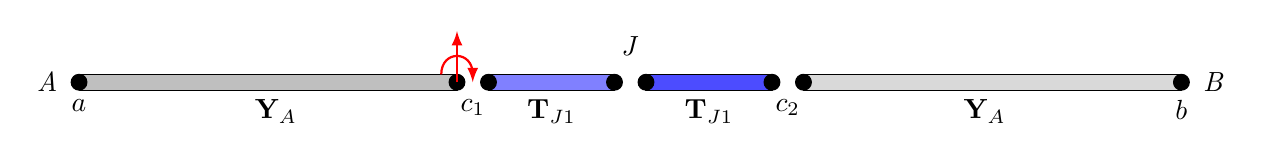
\begin{tikzpicture}[line join=round]
	% Top bar (A)
	\draw[fill=gray!50] (-3,0) rectangle (1.8,0.2);
	\draw[fill=blue!50] (2.2,0) rectangle (3.8,0.2);
	\draw[fill=blue!70] (4.2,0) rectangle (5.8,0.2);	% Bottom bar (B)
	\draw[fill=gray!30] (6.2,0) rectangle (11,0.2);
	
	\draw[fill] (-3,0.1) circle (0.1);
	\draw[fill] (1.8,0.1) circle (0.1);
	\draw[fill] (2.2,0.1) circle (0.1);	
	\draw[fill] (3.8,0.1) circle (0.1);	
	\draw[fill] (4.2,0.1) circle (0.1);	
	\draw[fill] (5.8,0.1) circle (0.1);	
	\draw[fill] (6.2,0.1) circle (0.1);
	\draw[fill] (11,0.1) circle (0.1);		
	
	\draw[thick,-latex,red] (1.8,0.1) --+ (0,0.65);
	
  \draw[-latex, draw=red, , thick] ($(1.8,0.1) +(-0.2,0.1)$) to [out=90,in=90, looseness=2] ($(1.8,0.1) +(+0.2,0.1)$) to ($(1.8,0.1) +(+0.2,0.)$);

				% Central post
%	\draw[fill=blue] (2.8,0.2) rectangle (3,1);
	% Labels
	\node[left]  at (-3.15,0.1)       {\textit{A}};
	\node[right]  at (11.15, 0.1)     {\textit{B}};
	\node[below] at (4,0.8)  {\textit{J}};
	
	\node[below]  at (-3,0)       {$a$};
	\node[below]  at (11,0)       {$b$};
	\node[below]  at (2,0)       {$c_1$};	
	\node[below]  at (6,0)       {$c_2$};	
	
			
	\node[below] at (-0.5,-0.)        {$\mathbf{Y}_{A}$};
	\node[below] at (3,-0.)        {$\mathbf{T}_{J1}$};
	\node[below] at (5,-0.)        {$\mathbf{T}_{J1}$};
	\node[below] at (8.5,-0.)        {$\mathbf{Y}_{A}$};
	\end{tikzpicture}
	
	\end{document}